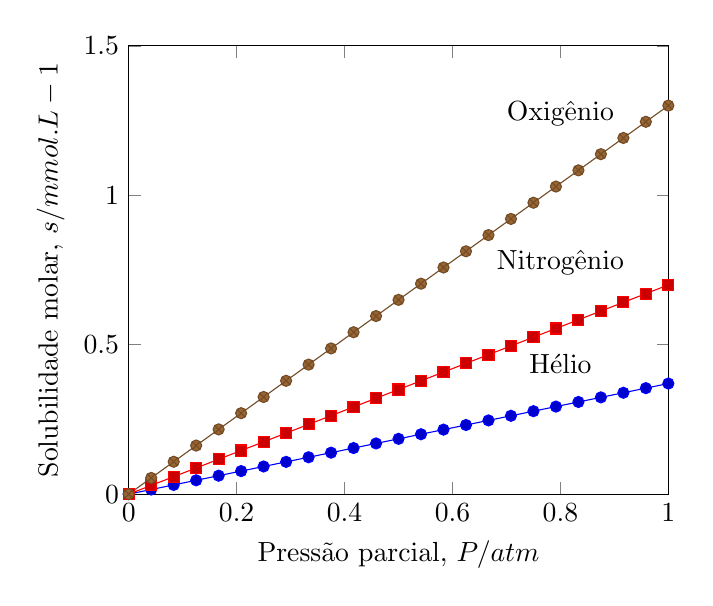
\begin{tikzpicture}
    \begin{axis}
        [
            grid = none,
            xlabel = {Pressão parcial, $P/\unit{atm}$},
            ylabel = {Solubilidade molar, $s/\unit{mmol.L-1}$},
            xmin = 0, xmax = 1,
            domain = 0:1,
            ymin = 0, ymax = 1.5,
        ]

    \addplot
        { 0.37 * x };

    \addplot
        { 0.70 * x };

    \addplot
        { 1.30 * x };

    \node [anchor = south] at (axis cs:0.8,1.2) 
        {Oxigênio};

    \node [anchor = south] at (axis cs:0.8,0.7) 
        {Nitrogênio};
        
    \node [anchor = north] at (axis cs:0.8,0.5) 
        {Hélio};

    \end{axis}
\end{tikzpicture}
